\chapter{Leçon 31: Konversatioun an enger Immobilienagentur}

Dës Lektioun beschäftegt sech mat enger Konversatioun an enger Immobilienagentur, wou eng Koppel (Chantal an Carlos) no enger gëeegenter Wunneng fir hir Famill sicht an Informatioune vum Agent kritt. Mir studéieren d'Aussprooch an d'Schreifweis vun de Vokaler \textbf{ei}, \textbf{éi}, \textbf{äi} an \textbf{ee}, déi oft verwiesselt ginn. Mir kucken och d'Ënnerscheeder tëscht de Verben \textbf{kucken}, \textbf{ukucken} an \textbf{nokucken}, d'Benotzung vum Numerus \textbf{zwou} fir feminin Substantiven, an de Kontrast tëscht \textbf{Knupp} an \textbf{Knippchen} (inklusive vum Ausdrock \textbf{déi geckeg Knippchen} fir de progressive Knach am Ielebou). \textit{Cette leçon porte sur une conversation dans une agence immobilière, où un couple (Chantal et Carlos) cherche un logement adapté pour sa famille et obtient des informations de l'agent. Nous étudions la prononciation et l'orthographe des voyelles \textbf{ei}, \textbf{éi}, \textbf{äi} et \textbf{ee}, qui sont souvent confondues. Nous analysons également les différences entre les verbes \textbf{kucken} (regarder), \textbf{ukucken} (regarder de près / visiter) et \textbf{nokucken} (vérifier / suivre du regard), l'utilisation du nombre \textbf{zwou} pour les noms féminins, et la distinction entre \textbf{Knupp} (butte / bosse) et \textbf{Knippchen} (praline / drôle de coude). / This lesson covers a conversation in a real estate agency, where a couple (Chantal and Carlos) looks for a suitable apartment for their family and gets information from the agent. We study the pronunciation and spelling of the vowels \textbf{ei}, \textbf{éi}, \textbf{äi}, and \textbf{ee}, which are frequently confused. We also examine the differences between the verbs \textbf{kucken} (to look), \textbf{ukucken} (to look at / inspect), and \textbf{nokucken} (to check / watch), the use of the number \textbf{zwou} for feminine nouns, and the contrast between \textbf{Knupp} (bump/hill) and \textbf{Knippchen} (praline / funny bone).}

\vspace{1em}

\section[Dialog: An der Immobilienagentur / Dialogue / Dialogue]{Dialog: An der Immobilienagentur \\/ Dialogue : À l'agence immobilière \\/ Dialogue: At the Real Estate Agency}

\noindent\textbf{Charakteren: M = D'Maklerin, S = Chantal, C = Carlos} \\
\textit{Note: Les rôles sont lus par la Maklerin (M), Chantal (S) et Carlos (C). / Note: The roles are read by the agent (M), Chantal (S), and Carlos (C).}

\vspace{1.5em}

\noindent\textbf{1. M: Moien, wëllkomm bei ImmoConsdorf. Wéi kann ech Iech hëllefen?}\\
\textit{Moien} (Bonjour / Hello), \textit{wëllkomm} (bienvenue / welcome) \textit{bei ImmoConsdorf} (chez ImmoConsdorf / at ImmoConsdorf). \textit{Wéi kann ech} (Comment puis-je / How can I) \textit{Iech hëllefen} (vous aider / help you)?\\
$\rightarrow$ Français : \textit{Bonjour, bienvenue chez ImmoConsdorf. Comment puis-je vous aider ?}\\
$\rightarrow$ English : \textit{Hello, welcome to ImmoConsdorf. How can I help you?}\\[0.5em]

\noindent\textbf{2. S: Moien, mir sichen eng Wunneng fir eis Famill. Mir hunn dräi Kanner, also brauche mir e bësse Plaz.}\\
\textit{Moien} (Bonjour / Hello), \textit{mir sichen} (nous cherchons / we are looking for) \textit{eng Wunneng} (un appartement, un logement / an apartment, a flat) \textit{fir eis Famill} (pour notre famille / for our family). \textit{Mir hunn} (Nous avons / We have) \textit{dräi Kanner} (trois enfants / three children), \textit{also brauche mir} (donc nous avons besoin de / so we need) \textit{e bësse Plaz} (un peu de place, d'espace / a bit of space, room).\\
$\rightarrow$ Français : \textit{Bonjour, nous cherchons un logement pour notre famille. Nous avons trois enfants, donc nous avons besoin d'un peu d'espace.}\\
$\rightarrow$ English : \textit{Hello, we are looking for an apartment for our family. We have three children, so we need a bit of space.}\\[0.5em]

\noindent\textbf{3. C: Ideal wieren dräi bis véier Schlofkummeren.}\\
\textit{Ideal} (Idéalement / Ideally) \textit{wieren} (seraient / would be) \textit{dräi bis véier} (trois à quatre / three to four) \textit{Schlofkummeren} (chambres à coucher / bedrooms).\\
$\rightarrow$ Français : \textit{Idéalement, trois à quatre chambres.}\\
$\rightarrow$ English : \textit{Ideally, three to four bedrooms.}\\[0.5em]

\noindent\textbf{4. M: Hutt Dir schonn eng Iddi vum Budget oder vum Quartier?}\\
\textit{Hutt Dir schonn} (Avez-vous déjà / Do you already have) \textit{eng Iddi} (une idée / an idea) \textit{vum Budget} (du budget / of the budget) \textit{oder vum Quartier} (ou du quartier / or of the neighborhood)?\\
$\rightarrow$ Français : \textit{Avez-vous déjà une idée du budget ou du quartier ?}\\
$\rightarrow$ English : \textit{Do you already have an idea of the budget or the neighborhood?}\\[0.5em]

\noindent\textbf{5. S: Mir géifen am léifsten zu Consdorf oder an der Géigend bleiwen, wéinst der Schoul.}\\
\textit{Mir géifen} (Nous aimerions, nous préférerions / We would like, we would prefer) \textit{am léifsten} (le plus volontiers, de préférence / preferably) \textit{zu Consdorf} (à Consdorf / in Consdorf) \textit{oder an der Géigend} (ou dans les environs, la région / or in the area) \textit{bleiwen} (rester / to stay), \textit{wéinst der Schoul} (à cause de l'école / because of the school).\\
$\rightarrow$ Français : \textit{Nous préférerions rester à Consdorf ou dans les environs, à cause de l'école.}\\
$\rightarrow$ English : \textit{We would prefer to stay in Consdorf or in the area, because of the school.}\\[0.5em]

\noindent\textbf{6. C: De Budget läit bei 1,2 bis 1,4 Milliounen.}\\
\textit{De Budget} (Le budget / The budget) \textit{läit bei} (se situe à, est de / lies at, is around) \textit{1,2 bis 1,4 Milliounen} (1,2 à 1,4 millions / 1.2 to 1.4 million).\\
$\rightarrow$ Français : \textit{Le budget est entre 1,2 et 1,4 millions.}\\
$\rightarrow$ English : \textit{The budget is between 1.2 and 1.4 million.}\\[0.5em]

\noindent\textbf{7. M: Ech hunn eng Wunneng mat 140 m², dräi Schlofkummeren, engem Balkon an engem klenge Gaart.}\\
\textit{Ech hunn} (J'ai / I have) \textit{eng Wunneng} (un appartement / an apartment) \textit{mat 140 m²} (de 140 mètres carrés / of 140 square meters), \textit{dräi Schlofkummeren} (trois chambres à coucher / three bedrooms), \textit{engem Balkon} (un balcon / a balcony) \textit{an engem klenge Gaart} (et un petit jardin / and a small garden).\\
$\rightarrow$ Français : \textit{J'ai un appartement de 140 m², trois chambres, un balcon et un petit jardin.}\\
$\rightarrow$ English : \textit{I have an apartment of 140 m², three bedrooms, a balcony, and a small garden.}\\[0.5em]

\noindent\textbf{8. S: Wou läit déi?}\\
\textit{Wou} (Où / Where) \textit{läit déi} (se trouve-t-il, se situe-t-il / is it located, does it lie)?\\
$\rightarrow$ Français : \textit{Où se trouve-t-elle ?}\\
$\rightarrow$ English : \textit{Where is it located?}\\[0.5em]

\noindent\textbf{9. M: Zu Consdorf, net wäit vun der Primärschoul.}\\
\textit{Zu Consdorf} (À Consdorf / In Consdorf), \textit{net wäit} (pas loin / not far) \textit{vun der Primärschoul} (de l'école primaire / from the primary school).\\
$\rightarrow$ Français : \textit{À Consdorf, pas loin de l'école primaire.}\\
$\rightarrow$ English : \textit{In Consdorf, not far from the primary school.}\\[0.5em]

\noindent\textbf{10. C: Wéi gesäit et mat Parking aus?}\\
\textit{Wéi gesäit et} (Comment cela se présente-t-il / How does it look) \textit{mat Parking} (avec le parking / with parking) \textit{aus} (separable prefix of \textit{ausgesinn}: \textit{wéi gesäit et aus mit} $\rightarrow$ qu'en est-il de / what about)?\\
$\rightarrow$ Français : \textit{Et pour le parking ? (Qu'en est-il du stationnement ?)}\\
$\rightarrow$ English : \textit{And what about parking?}\\[0.5em]

\noindent\textbf{11. M: Zwee Indoor-Parkingplazen an eng Cave.}\\
\textit{Zwee} (Deux / Two) \textit{Indoor-Parkingplazen} (places de parking intérieures / indoor parking spots) \textit{an eng Cave} (et une cave / and a cellar) \textit{[also: e Keller]}.\\
$\rightarrow$ Français : \textit{Deux places de parking intérieures et une cave.}\\
$\rightarrow$ English : \textit{Two indoor parking spots and a cellar.}\\[0.5em]

\noindent\textbf{12. S: Wéi al ass d'Gebai?}\\
\textit{Wéi al} (Quel âge / How old) \textit{ass d'Gebai} (est le bâtiment, l'immeuble / is the building)?\\
$\rightarrow$ Français : \textit{Et quel âge a le bâtiment ?}\\
$\rightarrow$ English : \textit{How old is the building?}\\[0.5em]

\noindent\textbf{13. M: Vun 2018, modern an energieeffizient.}\\
\textit{Vun 2018} (De 2018 / From 2018), \textit{modern} (moderne / modern) \textit{an energieeffizient} (et économe en énergie, efficace sur le plan énergétique / and energy-efficient).\\
$\rightarrow$ Français : \textit{De 2018, moderne et économe en énergie.}\\
$\rightarrow$ English : \textit{From 2018, modern and energy-efficient.}\\[0.5em]

\noindent\textbf{14. M: Den zweeten Objet ass 165 m², véier Schlofkummeren, eng grouss Terrass an eng modern Kichen.}\\
\textit{Den zweeten Objet} (Le deuxième bien, objet / The second property, object) \textit{ass 165 m²} (fait 165 mètres carrés / is 165 square meters), \textit{véier Schlofkummeren} (quatre chambres / four bedrooms), \textit{eng grouss Terrass} (une grande terrasse / a large terrace) \textit{an eng modern Kichen} (et une cuisine moderne / and a modern kitchen).\\
$\rightarrow$ Français : \textit{Le deuxième bien fait 165 m², quatre chambres, une grande terrasse et une cuisine moderne.}\\
$\rightarrow$ English : \textit{The second property is 165 m², four bedrooms, a large terrace, and a modern kitchen.}\\[0.5em]

\noindent\textbf{15. C: Dat kéint fir eis passen.}\\
\textit{Dat} (Cela / That) \textit{kéint} (pourrait / could) \textit{fir eis passen} (nous convenir, aller pour nous / suit us, fit us).\\
$\rightarrow$ Français : \textit{Cela pourrait nous convenir.}\\
$\rightarrow$ English : \textit{That could suit us.}\\[0.5em]

\noindent\textbf{16. S: Wou ass deen?}\\
\textit{Wou} (Où / Where) \textit{ass deen} (est celui-là / is that one)?\\
$\rightarrow$ Français : \textit{Où se trouve-t-il ?}\\
$\rightarrow$ English : \textit{Where is it?}\\[0.5em]

\noindent\textbf{17. M: Zu Iechternach, ongeféier 10 Minutte vun hei.}\\
\textit{Zu Iechternach} (À Echternach / In Echternach), \textit{ongeféier} (environ, à peu près / approximately, about) \textit{10 Minutte} (10 minutes / 10 minutes) \textit{vun hei} (d'ici / from here).\\
$\rightarrow$ Français : \textit{À Echternach, à environ 10 minutes d'ici.}\\
$\rightarrow$ English : \textit{In Echternach, about 10 minutes from here.}\\[0.5em]

\noindent\textbf{18. C: A wéi vill kascht deen?}\\
\textit{A wéi vill} (Et combien / And how much) \textit{kascht deen} (coûte-t-il / does that one cost)?\\
$\rightarrow$ Français : \textit{Et combien coûte celui-là ?}\\
$\rightarrow$ English : \textit{And how much does that one cost?}\\[0.5em]

\noindent\textbf{19. M: 1,45 Milliounen, verhandelbar.}\\
\textit{1,45 Milliounen} (1,45 million / 1.45 million), \textit{verhandelbar} (négociable / negotiable).\\
$\rightarrow$ Français : \textit{1,45 million, négociable.}\\
$\rightarrow$ English : \textit{1.45 million, negotiable.}\\[0.5em]

\noindent\textbf{20. S: Dat ass knapp iwwer eisem Budget, mee mir kucken eis en un.}\\
\textit{Dat ass} (C'est / That is) \textit{knapp} (tout juste, à peine / barely, just) \textit{iwwer eisem Budget} (au-dessus de notre budget / above our budget), \textit{mee} (mais / but) \textit{mir kucken eis} (nous nous regardons $\rightarrow$ nous visitons pour nous / we look at for ourselves) \textit{en un} (separable prefix of \textit{ukucken}: \textit{eppes unkucken} $\rightarrow$ visiter/regarder quelque chose / inspect/take a look at something).\\
$\rightarrow$ Français : \textit{C'est un peu au-dessus de notre budget, mais nous allons le visiter.}\\
$\rightarrow$ English : \textit{That is just over our budget, but we will take a look at it.}\\[0.5em]

\noindent\textbf{21. M: Soll ech Iech fir eng Visitt androen?}\\
\textit{Soll ech} (Dois-je, voulez-vous que je / Should I) \textit{Iech} (vous / you) \textit{fir eng Visitt} (pour une visite / for a visit) \textit{androen} (inscrire, enregistrer / register, sign up)?\\
$\rightarrow$ Français : \textit{Voulez-vous que je vous inscrive pour une visite ?}\\
$\rightarrow$ English : \textit{Should I sign you up for a visit?}\\[0.5em]

\noindent\textbf{22. S: Donneschdeg Nomëtteg géif eis passen.}\\
\textit{Donneschdeg Nomëtteg} (Jeudi après-midi / Thursday afternoon) \textit{géif} (conditionnel de \textit{ginn}: \textit{géif passen} $\rightarrow$ conviendrait / would suit, would fit) \textit{eis passen} (nous aller, nous convenir / suit us).\\
$\rightarrow$ Français : \textit{Jeudi après-midi nous conviendrait.}\\
$\rightarrow$ English : \textit{Thursday afternoon would suit us.}\\[0.5em]

\noindent\textbf{23. C: Jo, dat ass perfekt.}\\
\textit{Jo} (Oui / Yes), \textit{dat ass} (c'est / that is) \textit{perfekt} (parfait / perfect).\\
$\rightarrow$ Français : \textit{Oui, c'est parfait.}\\
$\rightarrow$ English : \textit{Yes, that is perfect.}\\[0.5em]

\noindent\textbf{24. M: Ech notéieren Donneschdeg. Ech schécken Iech d'Dossieren per E-Mail.}\\
\textit{Ech notéieren} (Je note / I note down) \textit{Donneschdeg} (jeudi / Thursday). \textit{Ech schécken Iech} (Je vous envoie / I send you) \textit{d'Dossieren} (les dossiers / the files) \textit{per E-Mail} (par e-mail / by email).\\
$\rightarrow$ Français : \textit{Je note jeudi. Je vous enverrai les dossiers par e-mail.}\\
$\rightarrow$ English : \textit{I will note down Thursday. I will send you the files by email.}\\[0.5em]

\noindent\textbf{25. S: Merci villmools.}\\
\textit{Merci villmools} (Merci beaucoup / Thank you very much).\\
$\rightarrow$ Français : \textit{Merci beaucoup.}\\
$\rightarrow$ English : \textit{Thank you very much.}\\[0.5em]

\noindent\textbf{26. C: Mir freeën eis op d'Visitten.}\\
\textit{Mir freeën eis} (Nous nous réjouissons / We look forward) \textit{op d'Visitten} (des visites / to the visits).\\
$\rightarrow$ Français : \textit{Nous nous réjouissons des visites.}\\
$\rightarrow$ English : \textit{We look forward to the visits.}\\[0.5em]

\noindent\textbf{27. M: Bis Donneschdeg.}\\
\textit{Bis Donneschdeg} (À jeudi / See you on Thursday).\\
$\rightarrow$ Français : \textit{À jeudi.}\\
$\rightarrow$ English : \textit{See you on Thursday.}

\vspace{1.5cm}
\color{geminiBlue}\hrule height 1.5pt \vspace{0.5em}\color{black}

\section[Grammaire an Ausdréck / Grammaire / Grammar]{Grammaire an Ausdréck \\/ Grammaire et Expressions \\/ Grammar and Expressions}

\subsection*{1. Aussprooch a Schreifweis: "ei", "éi", "äi", "ee"}

Am Lëtzebuergeschen sinn d'Ënnerscheeder tëscht dëse Vokalkombinatiounen fundamental. Si ginn dacks vun de Studenten (besonnesch mat däitschem oder franséischem Hannergrond) verwiesselt. Hei sinn d'Reegelen an d'Beispiller aus dem Dialog: \\
\textit{En luxembourgeois, les différences entre ces combinaisons de voyelles sont fondamentales. Elles sont souvent confondues par les apprenants. Voici les règles et exemples du dialogue : / In Luxembourgish, the differences between these vowel combinations are fundamental. They are often confused by learners. Here are the rules and examples from the dialogue:}

\begin{itemize}
    \item \textbf{ei} (prononcé comme le "ei" allemand ou "aï" en français / pronounced like the German "ei" or English "eye" - /aɪ/): \\
    \textit{Beispiller:} \textbf{bleiwen} (rester / to stay), \textbf{eisem} (notre / our), \textbf{nei} (nouveau / new).
    
    \item \textbf{éi} (prononcé comme un "é" fermé long ou légèrement diphtongué / pronounced as a closed long "é" or slightly diphthongized - /eɪ/ or /eː/): \\
    \textit{Beispiller:} \textbf{léifsten} (le plus volontiers / preferably), \textbf{véier} (quatre / four), \textbf{géif} (conviendrait / would), \textbf{zwéin} (deux / two - masc.).
    
    \item \textbf{äi} (prononcé comme un "a" très ouvert suivi de "i", similaire au "y" anglais dans "my" / pronounced as a very open "a" followed by "i", similar to the English "y" in "my" - /æɪ/): \\
    \textit{Beispiller:} \textbf{dräi} (trois / three), \textbf{läit} (se situe, de \textit{leien} / lies, is located), \textbf{Präis} (prix / price), \textbf{fräi} (libre / free), \textbf{däin} / \textbf{säin} (ton / son - your / his).
    
    \item \textbf{ee} (prononcé comme un "é" ou "è" long ou diphtongué en "e" muet / pronounced as a long "é" or "è" or diphthongized - /eː/ or /eə/): \\
    \textit{Beispiller:} \textbf{zweet} / \textbf{zweeten} (deuxième / second), \textbf{freeën} (réjouir / to look forward), \textbf{deementspriechend} (par conséquent / accordingly).
\end{itemize}

\subsection*{2. Kucken, Ukucken an Nokucken}

Den Dialog benotzt de Saz: \textit{"mee mir kucken eis en un"} (du Verb \textbf{sech eppes ukucken}). Hei sinn d'Ënnerscheeder an d'Konjugatioune vun dëse Verben: \\
\textit{Le dialogue utilise la phrase : "mee mir kucken eis en un" (du verbe "sech eppes ukucken"). Voici les différences et conjugaisons de ces verbes : / The dialogue uses the sentence: "mee mir kucken eis en un" (from the verb "sech eppes ukucken"). Here are the differences and conjugations of these verbs:}

\begin{itemize}
    \item \textbf{kucken} (regarder, observer - to look, to watch): \\
    S'utilise de manière générale. \\
    \textit{Beispill:} \textit{Ech kucke gär e Film.} (J'aime regarder un film. / I like watching a movie.)
    
    \item \textbf{ukucken} (regarder de près, contempler, visiter - to look at, to inspect): \\
    C'est un verbe séparable. Le préfixe \textbf{u-} va à la fin dans une proposition principale. \\
    \textit{Beispill:} \textit{Kuckt d'Foto un!} (Regardez la photo ! / Look at the photo!)
    
    \item \textbf{sech eppes ukucken} (visiter, examiner pour soi - to take a look at / inspect for oneself): \\
    C'est la forme réflexive avec un pronom d'objet (datif réflexif + accusatif). \\
    \textit{Beispill:} \textit{Mir kucken eis (datif) d'Wunneng (accusatif) un.} (Nous allons visiter / jeter un coup d'œil à l'appartement. / We are going to inspect the apartment ourselves.)
    
    \item \textbf{nokucken} (vérifier, chercher dans un dictionnaire, suivre du regard - to check, to look up, to watch someone leave): \\
    Également séparable. \\
    \textit{Beispill:} \textit{Kanns de d'Reegel am Buch nokucken?} (Peux-tu vérifier la règle dans le livre ? / Can you look up the rule in the book?)
\end{itemize}

\subsection*{3. Genus-Iwwerestëmmung beim Zuelenwuert "Zwee" (Gender agreement for the number two)}

Am Lëtzebuergeschen huet d'Zuel \textbf{zwee} dräi verschidde Forme jee no dem Genus (genre) vum Substantiv: \\
\textit{En luxembourgeois, le chiffre deux a trois formes différentes selon le genre du nom qui le suit : / In Luxembourgish, the number two has three different forms depending on the gender of the noun:}
\begin{itemize}
    \item \textbf{zwéin} fir maskulin Substantiven (e.g. \textit{zwéin Hären} - deux messieurs / two gentlemen).
    \item \textbf{zwou} fir feminin Substantiven (e.g. \textit{zwou Indoor-Parkingplazen} - deux places de parking / two parking spots). \\
    \textit{Note : Bien que dans le dialogue lu sur la feuille il y ait écrit "Zwee Indoor-Parkingplazen" (usage familier ou erreur fréquente), la forme grammaticale correcte et obligatoire est \textbf{zwou}, car "d'Parkingplaz" est un nom féminin. / Note: Although the sheet dialogue has "Zwee Indoor-Parkingplazen" written (a common colloquial usage or mistake), the correct and mandatory grammatical form is \textbf{zwou}, since "d'Parkingplaz" is a feminine noun.}
    \item \textbf{zwee} fir neutral Substantiven oder am Allgemengen (e.g. \textit{zwee Kanner} - deux enfants / two children).
\end{itemize}

\subsection*{4. Knupp an Knippchen}

\begin{itemize}
    \item \textbf{d'Knupp} (f., Pl.: \textit{Knuppen}): \\
    \textit{Français : Une butte, une colline, une bosse ou un tas (allemand : Hügel, Anhöhe, Beule). / English: A hill, a hill-top, a bump, or a lump (German: Hügel, Anhöhe, Beule).}
    
    \item \textbf{d'Knippchen} (f., Pl.: \textit{d'Knippercher}): \\
    \textit{Français : C'est le diminutif de \textbf{Knupp}. Outre le sens géographique de petite colline (comme la colline de la "Knippchen" à Arlon), ce mot désigne de manière autonome et très courante en luxembourgeois une \textbf{praline au chocolat} ! / English: It is the diminutive form of \textbf{Knupp}. Aside from the geographical meaning of a small hill or mound (such as the "Knippchen" hill in Arlon), this word is used independently in daily Luxembourgish to refer to a \textbf{chocolate praline}! }
    
    \item \textbf{déi geckeg Knippchen} (f., Pl.: \textit{déi geckeg Knippercher}): \\
    \textit{Français : C'est l'expression populaire pour le \textbf{petit coude} (le nerf ulnaire au niveau du coude, provoquant une sensation de décharge électrique lors d'un choc). / English: This is the popular idiomatic expression for the \textbf{funny bone} (the ulnar nerve at the elbow, which produces an electric-shock-like tingling sensation when bumped).}
\end{itemize}

\subsection*{5. Adjektivdeclinatioun virun feminine Substantiven (Adjective inflection before feminine nouns)}

Denkt un d'Reegel fir d'Adjektiver am feminine Singular nom onbestëmmten Artikel \textbf{eng}: \\
\textit{Rappelez-vous la règle d'accord de l'adjectif féminin singulier après l'article indéfini "eng" : / Remember the adjective inflection rule for feminine singular nouns after the indefinite article "eng":}
\begin{itemize}
    \item \textit{Français : Les adjectifs épithètes qualifiant un nom féminin singulier précédé de \textbf{eng} ne prennent aucune terminaison ! / English: Attributive adjectives modifying a feminine singular noun preceded by \textbf{eng} do not take any ending!}
    \item \textit{Beispill:} \textbf{eng geckeg Knippchen} (\textit{Français : une drôle de praline / a funny bone, et non pas \textit{eng geckegen Knippchen}. C'est l'application de la règle générale des adjectifs féminins singuliers (e.g. \textit{eng gedréckt Zäitung}). / English: a funny bone, and not \textit{eng geckegen Knippchen}. This is the application of the general adjective declension rule for feminine singular nouns (e.g., \textit{eng gedréckt Zäitung} - a printed newspaper, not \textit{eng gedréckten}).})
\end{itemize}

\vspace{1.5cm}
\color{geminiBlue}\hrule height 1.5pt \vspace{0.5em}\color{black}

\section[Vokabulär: Neit Wierderbuch]{Vokabulär: Neit Wierderbuch \\/ Nouveau Vocabulaire Illustré \\/ New Illustrated Vocabulary}

\begin{itemize}
    \item \textbf{d'Immobilienagentur} (f., Pl.: \textit{d'Immobilienagenturen}) $\rightarrow$ l'agence immobilière (the real estate agency)
    \item \textbf{d'Maklerin} (f., Pl.: \textit{d'Maklerinnen}) $\rightarrow$ l'agent immobilier (femelle) (the real estate agent - female)
    \item \textbf{de Makler} (m., Pl.: \textit{d'Makleren}) $\rightarrow$ l'agent immobilier (mâle) (the real estate agent - male)
    \item \textbf{d'Wunneng} (f., Pl.: \textit{d'Wunnengen}) $\rightarrow$ l'appartement, le logement (the apartment, the flat)
    \item \textbf{d'Schlofkummer} (f., Pl.: \textit{d'Schlofkummeren}) $\rightarrow$ la chambre à coucher (the bedroom)
    \item \textbf{de Gaart} (m., Pl.: \textit{d'Gäert}) $\rightarrow$ le jardin (the garden)
    \item \textbf{de Balkon} (m., Pl.: \textit{d'Balkonen}) $\rightarrow$ le balcon (the balcony)
    \item \textbf{d'Terrass} (f., Pl.: \textit{d'Terrassen}) $\rightarrow$ la terrasse (the terrace)
    \item \textbf{d'Kichen} (f., Pl.: \textit{d'Kichenen}) $\rightarrow$ la cuisine (the kitchen)
    \item \textbf{d'Cave} (f., Pl.: \textit{d'Caven}) $\rightarrow$ la cave (the cellar)
    \item \textbf{de Keller} (m., Pl.: \textit{d'Kelleren}) $\rightarrow$ la cave, le cellier (the cellar)
    \item \textbf{d'Gebai} (n., Pl.: \textit{d'Gebaier}) $\rightarrow$ le bâtiment, l'immeuble (the building)
    \item \textbf{de Budget} (m., Pl.: \textit{d'Budgeten}) $\rightarrow$ le budget (the budget)
    \item \textbf{de Präis} (m., Pl.: \textit{d'Präisser}) $\rightarrow$ le prix (the price)
    \item \textbf{d'Knupp} (f., Pl.: \textit{d'Knuppen}) $\rightarrow$ la butte, la colline (the bump, the hill)
    \item \textbf{d'Knippchen} (f., Pl.: \textit{d'Knippercher}) $\rightarrow$ la praline en chocolat, la petite butte (the chocolate praline, the small hill)
    \item \textbf{déi geckeg Knippchen} (f., Pl.: \textit{déi geckeg Knippercher}) $\rightarrow$ le petit coude (funny bone)
    \item \textbf{zwou} (num.) $\rightarrow$ deux (pour noms féminins) (two - feminine)
    \item \textbf{bleiwen} (v.) $\rightarrow$ rester (to stay)
    \item \textbf{verhandelbar} (adj.) $\rightarrow$ négociable (negotiable)
    \item \textbf{energieeffizient} (adj.) $\rightarrow$ économe en énergie (energy-efficient)
\end{itemize}

\vspace{1.5em}

\begin{center}
    \begin{minipage}[t]{0.48\textwidth}
        \centering
        \textbf{Eng Wunneng}
        \vspace{0.5em}
        \framebox{\parbox{0.9\linewidth}{\centering
            \vspace{0.5cm}
            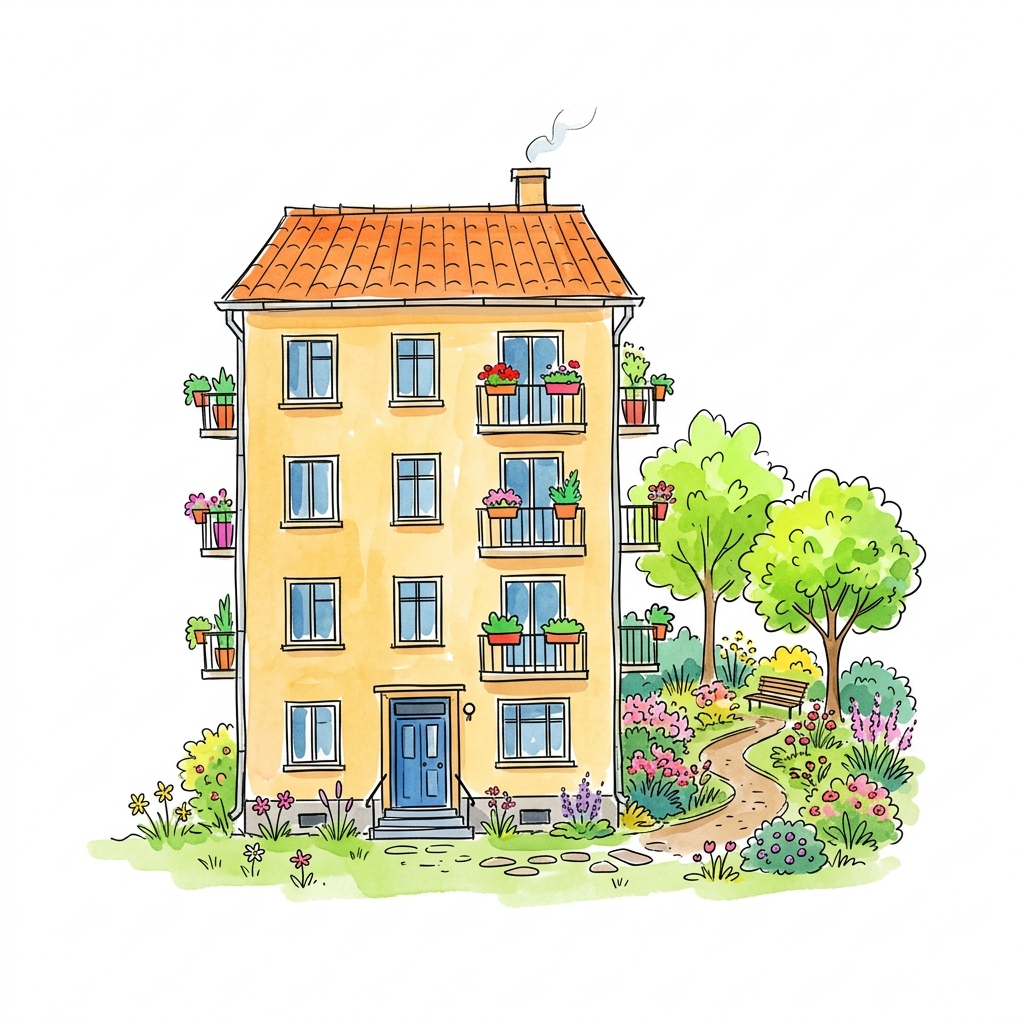
\includegraphics[width=0.9\linewidth]{vokab_300dpi/wunneng.png} \\
            \small\textit{D'Wunneng (L'appartement / The apartment)}
            \vspace{0.5cm}
        }}
    \end{minipage}
    \hfill
    \begin{minipage}[t]{0.48\textwidth}
        \centering
        \textbf{Eng Knippchen}
        \vspace{0.5em}
        \framebox{\parbox{0.9\linewidth}{\centering
            \vspace{0.5cm}
            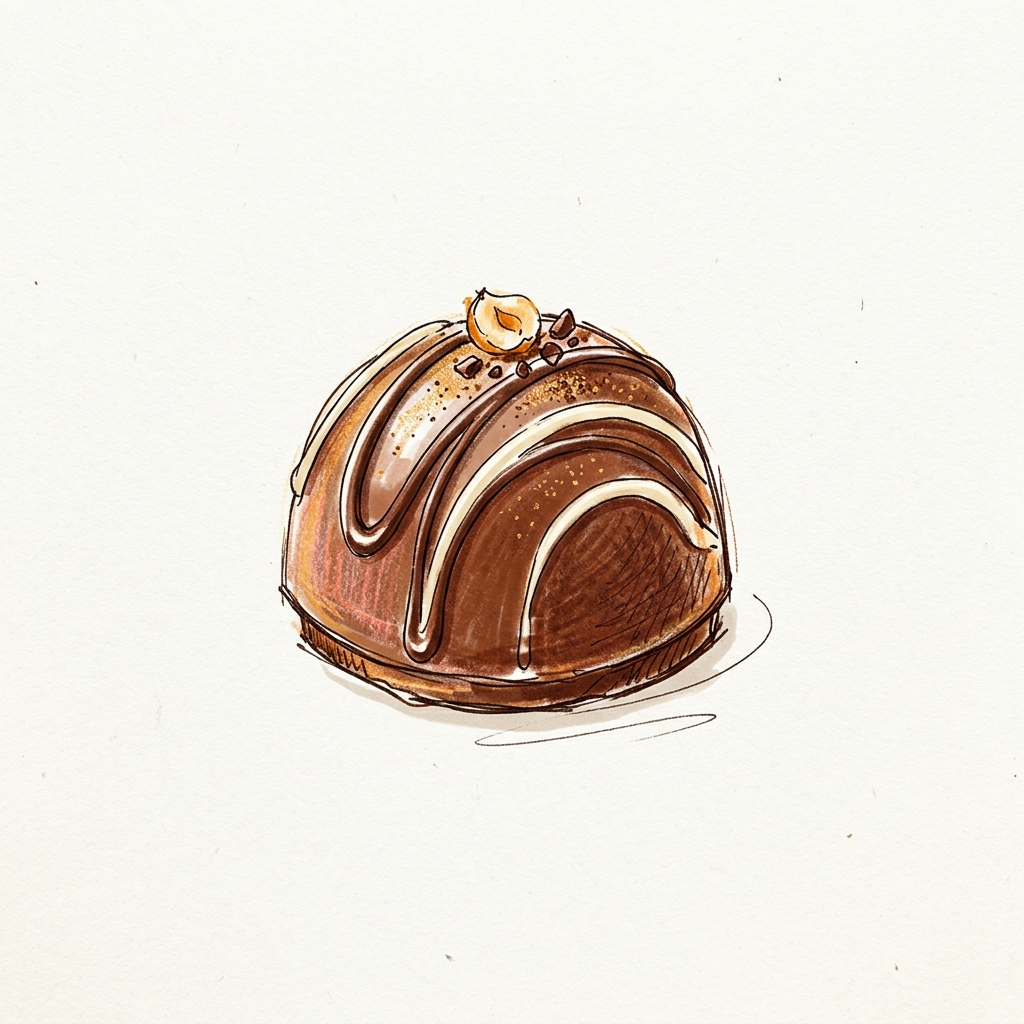
\includegraphics[width=0.9\linewidth]{vokab_300dpi/knippchen.png} \\
            \small\textit{D'Knippchen (La praline / The chocolate praline)}
            \vspace{0.5cm}
        }}
    \end{minipage}
    
    \vspace{1.5em}
    
    \begin{minipage}[t]{0.48\textwidth}
        \centering
        \textbf{Eng Knupp}
        \vspace{0.5em}
        \framebox{\parbox{0.9\linewidth}{\centering
            \vspace{0.5cm}
            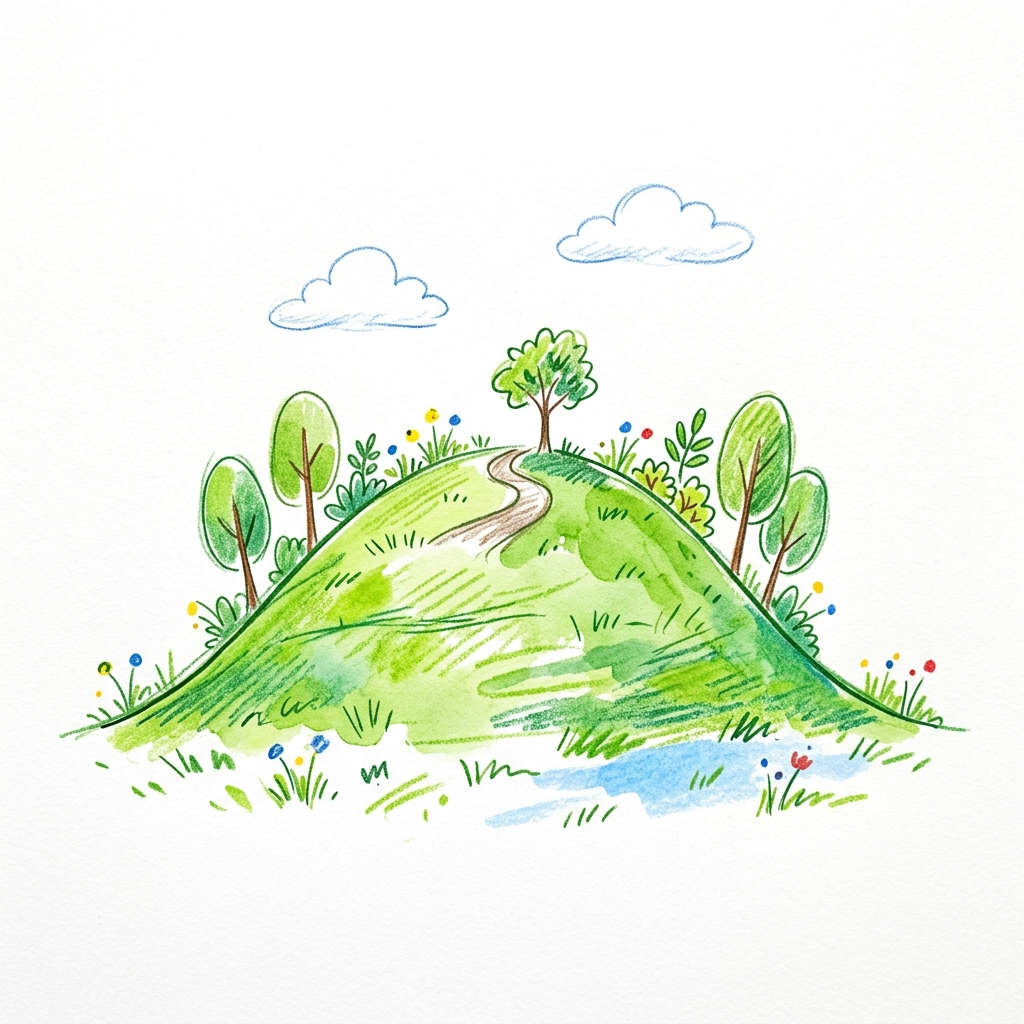
\includegraphics[width=0.9\linewidth]{vokab_300dpi/knupp.png} \\
            \small\textit{D'Knupp (La butte / The small hill)}
            \vspace{0.5cm}
        }}
    \end{minipage}
    \hfill
    \begin{minipage}[t]{0.48\textwidth}
        \centering
        \textbf{Eng geckeg Knippchen}
        \vspace{0.5em}
        \framebox{\parbox{0.9\linewidth}{\centering
            \vspace{0.5cm}
            
\includegraphics[width=0.9\linewidth]{vokab_300dpi/geckeg_knippchen.png} \\
            \small\textit{Déi geckeg Knippchen (Le petit coude / The funny bone)}
            \vspace{0.5cm}
        }}
    \end{minipage}
\end{center}
